\documentclass[12pt]{article}
%%%%%%%%%%%%%%%%%%%%%%%%%%%%%%%%%%%%%%%%%%
\usepackage{amsmath}
\usepackage[margin=1in]{geometry}
\usepackage{tabu}
\usepackage{makecell}
\usepackage[siunitx, american]{circuitikz}

\usepackage{graphicx}
\usepackage{caption}

\usepackage{tikz}
\usepackage{pgfplots}
\pgfplotsset{compat=newest}

\newcommand{\ohm}{$\Omega$}
\tabulinesep=1.2mm
%%%%%%%%%%%%%%%%%%%%%%%%%%%%%%%%%%%%%%%%%%

\title{ECE 3 Final Report}
\author{Kameron Carr \\ 504988167 \and Hien Ho \\ 505190709}
\date{TA: Xin Li \\ Section 1A \\ June 15, 2019}

\begin{document}
\maketitle

%1
\section{Introduction and Background}
The goal of this project if to use knowledge from the course to program a small car to follow a path designated by a black line within a given amount of time. As an additional part of the project, you must read data from the shaft encoders to more precisely control the speed of the car.
\\ 
The car must determine its error from the the center of the path can correct itself. This is done by using two feedback loop controllers. One is a linear controller so it simply takes the difference between where it is and where it wants to be in order to make adjustments. For example, if I am to the right of the line, turn left. The second is the derivative controller. This one looks at how its position is changing to make adjustments. For example, if I am drifting left, turn right. These two controllers can give the car different suggestions on which way to turn. Taking the sum of the two controller values can give the car a good sense of what adjustments need to be made.
\\ 
The path following system uses IR LEDs to shine light onto the ground, then the IR sensors detect how much light reflects off the ground below it to determine if the ground is black or white.
%IR Sensor Schematic
\begin{figure}[h]
  \begin{center}
  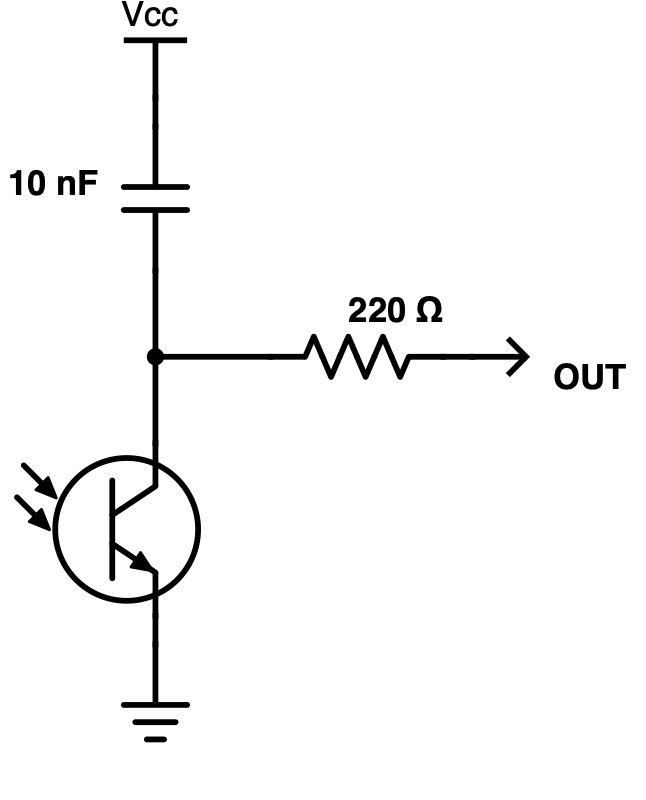
\includegraphics[width=0.2\linewidth]{IR-Sensor.png}
  \caption{Schematic for IR sensor \\ Source: Digi-Key Scheme-It online tool}
  \label{fig:sensor}
  \end{center}
\end{figure}
\\ 
As you can see in Figure \ref{fig:sensor}, the path sensor uses a resistor, capacitor, and phototransistor to detect IR light. When you put the sensor into output mode and set it to high, the out port becomes an in port and is set to $V_{cc}$. Therefore the voltage across the capacitor becomes 0V as long as you give it enough time. Upon changing the sensor pin to input mode, charge flows through the phototransistor depending on how much light is detected. This means that the voltage read on the pin will start at $V_{cc}$ and decay to zero over time. The rate of this decay depends on the amount of IR light entering the phototransistor.
%Example Curves
\begin{figure}[h]
  \begin{center}
  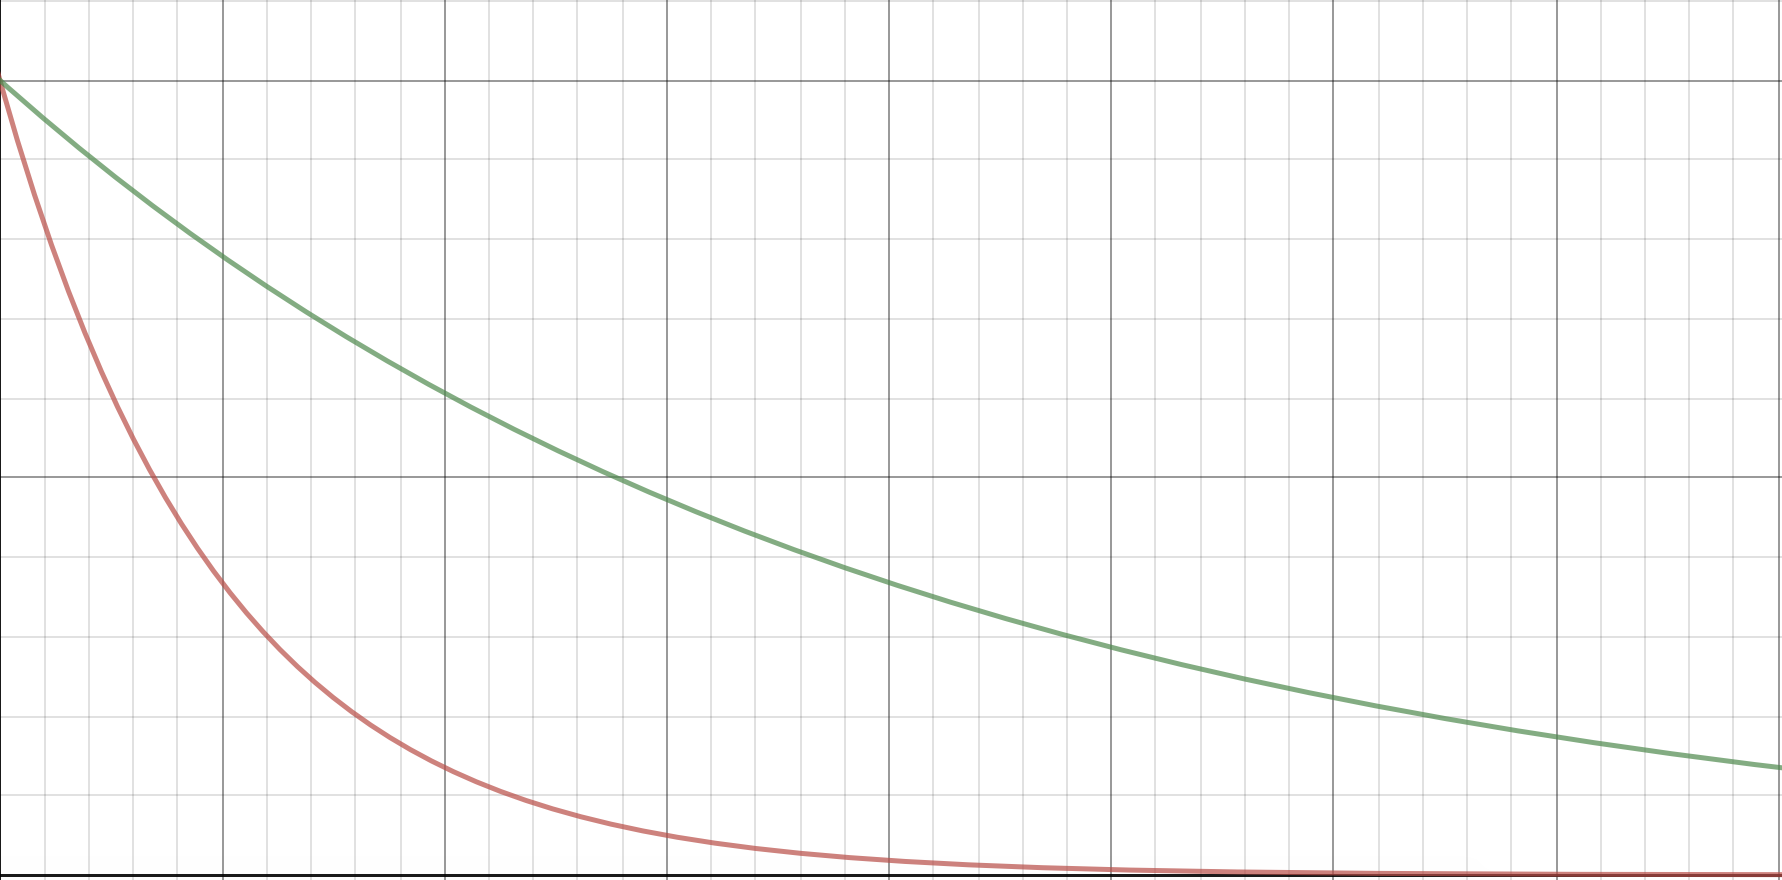
\includegraphics[width=0.5\linewidth]{curves.png}
  \caption{Example decay curves \\ Source: Desmos.com}
  \label{fig:curves}
  \end{center}
\end{figure}
In Figure \ref{fig:curves} you can see what the curves may look like for different amounts of IR light going into the phototransistor. The red curve represents if more light is going into the phototransistor and the green curve represents less light. The difference in voltages after a certain amount of time is what allows the sensor to read in either a 1 or a 0 depending on how much IR light ground below it reflects.

%2
\section{Testing Methodology}
%%2.1
\subsection{Motors}
%%%2.1.1
\subsubsection{Test Setup}
To start, you may need to assemble your car. This process includes assembling the wheels, putting the motors into the clamps on the car, and putting the LaunchPad on the car. You may need a TA's help to solder the header connections. Also it is important to remove the 5V jumper on the LaunchPad. If you are using the same car as the one used in this lab, not removing the jumper \textbf{may cause permanent damage to the car when plugging into a computer}. Also make sure to put fresh batteries in your car and turn it on using the switch on the back end.
\\
In order to be able control the motors in Energia, we first looked up the pin numbers on the MSP432 Pin Chart. From this chart we were able to find all the relevant pins to control the motors.
\\ \\
%%%Pin Chart
\begin{tabu}{|c|c|c|}
\hline
\textbf{Pin Functionality} & \textbf{Pin Number for Left Motor} & \textbf{Pin Number for Right Motor} \\ \hline
No Sleep (nSLP) & 31 & 11 \\
Direction (DIR) & 29 & 30 \\
Duty Cycle (PWM) & 40 & 39 \\
\hline
\end{tabu}
\\ \\ \\
Some of these pins also needed to be set to the correct mode and values. In Energia, the modes are set with the \texttt{pinMode} function, and the pin value is set through the \texttt{digitalWrite} function.
\\ \\
%%%Pin Values
\begin{tabu}{|c|c|c|}
\hline
\textbf{Pin Functionality} & \textbf{Pin Mode} & \textbf{Pin Value} \\ \hline
No Sleep (nSLP) & OUTPUT & HIGH \\
Direction (DIR) & OUTPUT & HIGH \\
\hline
\end{tabu} \\ \\
%%%2.1.2
\subsubsection{How the Tests were Conducted}
Knowing that the power to the motors ranges from 0-255, we wanted to get a feel for how fast the car went at different power levels. These are only rough guidelines of what we found to be true for our car. Note that these speeds can fluctuate depending on your car and the charge of your batteries. If you want to control the speed of the car with more precision, you must use the motor shaft encoders to measure the rotations.
\\ \\
%%%Motor Speeds
\begin{tabu}{|c|c|}
\hline
\textbf{Car Speed} & \textbf{Motor Power} \\ \hline
Not Moving &  0 - 20 \\
Slow       & 20 - 40 \\
Medium     & 40 - 90 \\
Fast       & 90 - 255 \\ \hline
\end{tabu}
\\ \\
Next we tested the evenness / straightness of the motors. We wanted to ensure that the car drove as straight as possible at the base power we would use in our path following program. Knowing the length of the course and the time limit, we were able to estimate that for our car to go fast enough, the base power of the motors would have to be around 60 on each motor. This is the target power we used when testing straightness. We noticed that going from zero power immediately to the target power would cause the car to jerk very quickly. For this reason, we used a for loop that changed the power of the motor incrementally with a small delay. This allowed the car to accelerate slowly and evenly without jerking around. We found this gave the most accurate results when trying to determine what power on each motor was needed to get the car to go straight.
\\ \\
%%%Motor Straightness
\begin{tabu}{|c|c|c|}
\hline
\textbf{Left Motor Power} & \textbf{Right Motor Power} & \textbf{Result} \\ \hline
62 & 60 & Pulled Right \\
60 & 60 & Straight \\
60 & 62 & Pulled Left \\ \hline
\end{tabu}

%%%2.1.3
\subsubsection{Data Analysis}
From these tests we found that the motors must have power of at least 20 to move consistently. A base power above 90 was found to be quite fast. We suspect a speed above this would make it significantly more difficult to respond to input from the path sensors and make appropriate adjustments.
\\ \\ 
We also found that our car goes straight when the power of each motor is set to 60. This suggests that the car will go straight unless the power of the motors is different.

%%%2.1.4
\subsubsection{Test Data Interpretation}
From these tests, we generally deduced that the motors were functioning as expected. By observing the general speeds of the motors at different power levels, we determined that a base power of 60 or greater would be a good starting goal for our car to finish the track in time. Also when using the shaft encoders to determine the speed of the vehicle, it is important to not go below 20 power on the motors, otherwise the feedback loop breaks because the motors are not turning. If the motors are not turning, the shaft encoders will not return information that can be used to calculated the speed.
\\ \\ 
The tests on motor straightness showed that our motors went at the same speed when the powers were equal. Therefore we did not include a bias value in our final code.

%%2.2
\subsection{Path Sensors}
%%%2.2.1
\subsubsection{Test Setup}
As with the motors, testing the path sensors requires the car to have the batteries put in and the switch turned on.
\\ 
In order to see the values from the sensors, we will need to be able to print to the serial monitor. The serial monitor must be initialized using \texttt{Serial.begin} and a data rate of 9600 bps.
\\ 
To get readings from the sensors, we need to initialize the pins for the sensors as well as the infrared LEDs. We look at the pin chart to find the pin values we can use in Energia to refer to the LEDs and sensors.
\\ \\ 
%Sensor Pins
\begin{tabu}{|l|c|}
\hline
\makecell{\textbf{Device}} & \textbf{Pin Number} \\ \hline
Sensor 0 (Right Most) & 65 \\
Sensor 1              & 48 \\
Sensor 2              & 64 \\
Sensor 3              & 47 \\
Sensor 4              & 52 \\
Sensor 5              & 68 \\
Sensor 6              & 53 \\
Sensor 7 (Left Most)  & 69 \\
IR LEDs (Odd)         & 45 \\
IR LEDs (Even)        & 61 \\ \hline
\end{tabu}
\\ \\ \\ 
All of the LEDs are set to \texttt{OUTPUT} using the \texttt{pinMode} function and to \texttt{HIGH} using the \texttt{digitalWrite} function.

%%%2.2.2
\subsubsection{How the Tests were Conducted}
To get readings from the sensors, we created a for loop that goes through the 8 sensors. For each sensor, you first have to set it to \texttt{OUTPUT} and \texttt{HIGH} then delay for 10 ms to charge the capacitor in the sensor. Then you set the sensor to \texttt{INPUT} and delay for a set amount of time before getting a reading using the \texttt{digitalRead} function. We tested a few values for this second delay. We did this by running the program and printing the sensor values to the serial monitor with the \texttt{Serial.print} function. We then moved the car side to side over a paper with a black line printed on it.
\\ \\ 
%Sensor Delays
\begin{tabu}{|c|c|}
\hline
\textbf{Delay} & \textbf{Behavior} \\ \hline
4 ms & All Zeros \\ 
3 ms & Some Incorrect Zeros \\ 
2 ms & Correct \\ 
1 ms & Correct \\ 
\hline
\end{tabu}

%%%2.2.3
\subsubsection{Data Analysis}
The car properly identified the difference between the white paper and the black printed paper when the delay after turning a sensor to input was 1 or 2 ms. A delay greater than 2ms resulted in unexpected / incorrect results. The errors were when the value should have been 1 but was instead 0. This is expected as if the delay is too large, then the capacitor will have too much time to discharge.

%%%2.2.4
\subsubsection{Test Data Interpretation}
Originally we took these results and decided that 2ms would be a good delay to have for our path following program. However, later when we tried sensing the horizontal black lines for the purpose of turning around or stopping, we found that a delay of 1 ms resulted in more accurate results.

%3
\section{Results and Discussion}
%%3.1
\subsection{Test Results}

%%3.2
\subsection{Race Day Results}

%4
\section{Conclusions and Future Work}

%5
\section{Illustration Credits}

%6
\section{References}


\end{document}
